\documentclass[amsart, 12pt]{article}
\usepackage{amsmath, amsthm, amssymb, amsfonts, textcomp}
\usepackage{graphicx}
\usepackage{float}
\title{Design and Implementation of OCR Text Correction by Crowdsourcing on Historic Newspaper Archive}
\author{Student Name: Megha Gupta\\
IIIT-D-MTech-CS-DE-13-MT11024\\
Indraprastha Institute of Information Technology,
New Delhi\\
\\
Advisor: Dr. Haimonti Dutta* \\
Co-Advisor: Manoj Pooleery* \\
*Affiliated to The Center for Computational Learning Systems,\\
Columbia University, New York\\
\\
Submitted in partial fulfillment of the requirements\\
for the degree of MTech in Computer Science\\
with Specialization in Data Engineering\\}


\begin{document}
\maketitle
\newpage
\section{Abstract}
Newspapers are the first draft of history, they have always been a rich source of information for historians, lay researchers, scholars, etc. With the advent of digitized newspapers, its accessibility to the general public has increased. 
The usability of these old historic newspapers has tremendously increased owing to OCR devices. However the text generated from the OCR devices is often garbled, affecting the efficiency of the retrieved results.\\
Our goal is to create a web based project that allows a patron to read and edit the articles. The task for editing the electronically translated newspapers is crowdsourced. This crowd based project would help in correcting the OCR errors thus improving the efficiency of retrieved results.\\
This report describes the OCR Text Correction System, its functions and workflow in section 2 and 3. Section 4 and 5 elaborates on its design model, System specifications and provides the steps to set up the code base. Implementation details with real screenshots and the challanges faced during development are mentioned in Section 6.

\newpage
\tableofcontents

\newpage
\section{Introduction}

\subsection{Problem Description}
This is a web based crowdsourcing project where patrons can edit the electronically translated or OCR-ed text of old historic newspapers present in the holdings of California Digital Newspaper Collection (CDNC) \cite{cdnc}. The OCR-ed text is often garbled due to inaccurate OCR devices. The accuracy of a device depends on the following factors: variations in the quality of input paper, size and style of font, column layout, etc. In our case, the quality of input paper is very poor as the newspapers date back to 1846. This adversely affects the retrieval effectiveness, hence the techniques for cleaning the OCR \cite{OCR} need to be improvised. Often such techniques involve laborious and time consuming manual processing of data. By correcting the garbled text, we will be able to improve the retrieved results thus making our users satisfied. \\

\subsection{Scope \& Objectives}
The objective of this project is to build a software that is usable, intuitive, simple and functions well consistently. It utilizes the \textgravedbl Wisdom of the Crowd\textacutedbl to gather information about the historical newspaper articles and magazines, and utilize Machine Learning for further analysis of data.\\
Our main focus here is on developing a web interface equipped with a text correction tool for enabling the users to correct the OCR errors as they come across them. By crowdsourcing this project, we accomplish more with fewer resources and build a user community in process.\\
The software is responsible for a host of functions. Its basic functions are searching and displaying images of issues, search by issue name and date range, user management functions, text correction functionality.\\
\subsection{Software Functions}
The project functions can be categorized into the following:
\begin{itemize}
\item User management functions \\
These encompass all the activities to manage the users for the application.  These include: \\
1.	Registration module: Ability to enter and validate user demographic information \\
2.	User Security module: Ability to authenticate and authorize the user \\
3.	User tracking module: Ability to track user activity, prepare statistics (how long users spent on each module, how many articles they corrected, participation in discussions etc) \\

\item Article related functions \\
1.	Articles search: this provides the capability to retrieve an article based on a set of criteria like article topic, date range etc. \\
2.	OCR correction: this interface provide users with the capability to correct the OCR displayed along side a given article image.  A basic level of authentication (based on a CAPTCHA model) will be required before the user can correct the text. \\
3.	Tag specification: this interface will allow the user to specify tags corresponding to a given article.  This functionality will also require a basic level of authentication. \\

\item Application administration functions
\end{itemize}
\section{Software Project Plan}

This project was divided into three phases: \\
Phase 1 included laying out UI components, database connectivity, searching and displaying user requested issues with their images. \\
Phase 2 included basic functionality text correction tool, user maagement functions. \\
Phase 3 included advance searching and functionality of tool. \\

\subsection{Workflow of the System}
\begin{itemize}
    \item In Phase 1, the first task was to design and build the layout of the interface. The user interface components in Vaadin can roughly be divided in two groups: components that the user can interact with and layout components for placing the other components to specific places in the UI. We started by creating a content layout for the UI, and then added the other layout components hierarchically, and finally the interaction components as the leaves of the component tree.\\
The Root Layout in this project is the Vertical Layout which encompasses two Horizontal Layouts, called mainLayout for the search options and the other called as bottomLayout. The bottomLayout is again divided into three panels called tool panel, image panel and function panel at left, center and right side of the screen respectively. The tool panel consists of tables, text correction tool, etc. The image panel consists of newspaper's images. And the function panel contains the user management controls.

\item Then we had to incorporate the basic search functionality on the basis of issue names given in the combobox, using date range from the date picker.
Once a issue is selected from the dropdown list and the search button is clicked, we get all the headlines of the selected issue in a table in the tool panel. And the images of the corresponding issue is displayed in the image panel. The headlines are in the form of links which when clicked shows the entire article in the table itself.
\item In Phase 2, the actual implementation of collaborative text correction tool takes place. Once we get the entire OCR text in the rows of a table, it also gets highlighted in the image at the image panel. Once \textgravedbl Edit Text\textacutedbl button is clicked, the OCR text becomes editable and a save button is displayed at the bottom of the left hand pane. A user can correct the text in the left panel to match it with the text in the image. 
\item Once the \textgravedbl Save\textacutedbl button is clicked, a check is performed against the database to determine which lines of text have been changed.  Only those text lines that have been changed are saved as a new version.
\item In Phase 3, we incorporate user management funcions, advance search options like phrase searching, enhance UI features and other functionalities of the tool.
\end{itemize}

\section{Design Models}
\subsection{Database Design}

The database design of our project is as given below.\\
\begin{figure}[ht!]
\centering
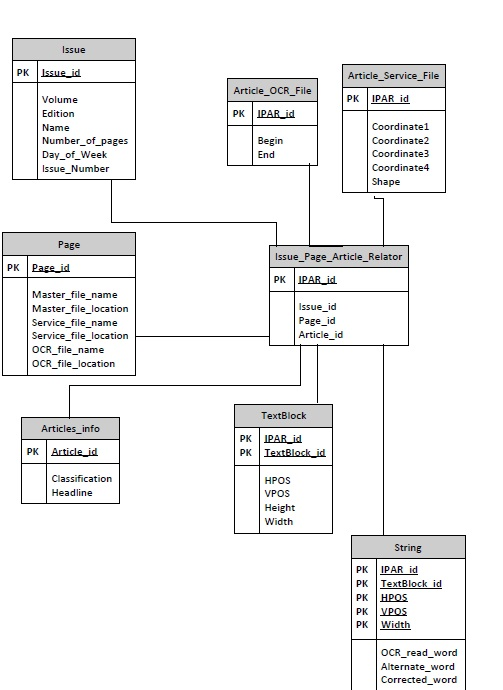
\includegraphics[width=10cm,height=10cm]{C:/Users/Megha/Documents/LEdProjects/ScholarlyMT11024/diag.jpg}
\caption{Database Design}
\label{fig:Phase 2}
\end{figure}

Following are the steps to access the Database Server (Postgres) using a command line client:
\begin{enumerate}
\item To connect to the database on Tesla.ldeo.columbia.edu, a tunnel needs to be established. To do this, type \\
ssh -Nn -L 5555:localhost:5432 username@tesla.ldeo.columbia.edu \& \\
where username is the corresponding user's name.
\item Open psql command line client and type in the following details:
Server [localhost] : localhost \\
Database [postgres]: nypltest \\
Port [5432]: 5555 \\
Username [postgres]: nypl\_user \\
password for nypl\_user: c9MamuaT \\
\item Commands like $\backslash$l and $\backslash$d gives the list of Databases and Relations in PostgreSQL.
\end{enumerate}
We have used views to access the tables present in the database. A View is a virtual table containing fields from one or more real tables. They make information retrieval fast and secure.\\
Following Views are used by our front end:
\begin{itemize}
\item vw\_issu\_page\_files \\
To get the page file locations (and related data) related to particular issue using the 'date\_of\_issue' column.

\item vw\_issue\_articles \\
To access all the articles related to a particular issue using the 'date\_of\_issue' column.

\item vw\_image\_info \\
To access the coordinates, shapes and related data for each article using the 'ipar\_id' column.

\item vw\_article\_text \\
To access entire text related to a particular article using the 'ipar\_id' column
\end{itemize}
\subsection{Architectural Design}
The architectural style that suits this project is the Model-View-Controller (MVC) architecture. It is the software architecture pattern that seperates the representation of information from user's interaction with it. It is used by applications that need the ability to maintain multiple views of the same data. The interaction between the three components is defined as: \\

\begin{itemize}
\item A controller sends commands to its associated view to change the view's presentation of the model. It can also send commands to the model to update the model's state. It processes every request, prepares other parts of the system like model and view.

\item A model handles data processing and database works part. It processes events sent by controller. After processing these events, it sends processed data to controller (thus, controller may reprocess it) or directly to view side allowing them to produce updated output.

\item A view prepares interface to show to the user.It requests from the model the information that it needs to generate an output representation to the user.\\
\end{itemize}
\begin{figure}[ht!]
\centering
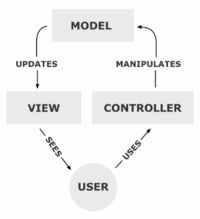
\includegraphics[width=9cm,height=7cm]{C:/Users/Megha/Documents/LEdProjects/ScholarlyMT11024/mvc.jpg}
\caption{MVC Architecture}
\label{fig:Phase 2}
\end{figure}

\subsubsection{Architectural Description}
In our project, we have MainWebApp.java as the controller which receives calls from the user and calls the relevant screen (model or view) based on the input.\\
Then we have IssueDisplay.java which acts as a view. This class is the primary display page for an issue, one page at a time.  It takes in the following parameters - list of articles in an issue and the page image to be displayed first.
It then display the list of articles as hyperlinks in the left pane, along with the issue title and display the image in the right pane. \\
Then we have DatabaseHelper.java which acts as a model containing any database objects that needs representation.


\section{System Study}
\subsection{Hardware Specification}
\begin{itemize}
    \item 32-bit Operating System 
\item 4GB RAM 
\item Intel(R) Core(TM) i3 CPU @ 2.13 GHz
\end{itemize}

\subsection{Software Specification}
\begin{itemize}
\item Eclipse Juno 4.2 IDE \\
It is an Integrated Development Environment (IDE) comprising of a base workspace and an extensible plug-in system for customizing environment. It is used to develop applications primarily in Java and other languages by means of other plug-ins.\\
We used the Vaadin plug-in to create our project in Eclipse Juno.

\item Vaadin 6 (Java Framework) plugin for Eclipse \\
It is an open source web application for rich Internet applications. It has server side architecture which means that the majority of the logic runs on the server. Ajax technology is used at the browser side to ensure a rich and interactive user experience. On the client-side Vaadin is built on top of Google Web Toolkit (GWT).\\
It uses Java as the programming language for creating web content. The framework incorporates event-driven programming and widgets.

\item Apache Tomcat 7.0.35
It is an open source web server and servlet container developed by the Apache Software Foundation (ASF). It implements the Java Servlet and the JavaServer Pages (JSP) specifications from Sun Microsystems, and provides a \textgravedbl pure\textacutedbl Java HTTP web server environment for Java code to run in. \\
It includes tools for configuration and management, but can also be configured by editing XML configuration files.

\item Apache Ant 1.8.4
It is a software tool for automating software build processes. It is similar to \textasciigrave Make\textasciiacute but is implemented using the Java language, requires the Java platform, and is best suited to building Java projects.\\
The most immediately noticeable difference between Ant and Make is that Ant uses XML to describe the build process and its dependencies, whereas Make uses Makefile format.

\item PostgreSQL
It is an open source object-relational database management system (ORDBMS) available for many platforms including Linux, Microsoft Windows and Mac OS X. \\
It implements the majority of the SQL:2008 standard, is ACID-compliant, is fully transactional (including all DDL statements), has extensible data types, operators, index methods, functions, aggregates, procedural languages, and has a large number of extensions written by third parties.

\item Tortoise SVN 1.7, A Subversion client for Windows
It is a free software that helps programmers manage different versions of the source code for their programs.Tortoise SVN is a Subversion client, implemented as a Microsoft Windows shell extension. It is released under the GNU General Public License.

\item Web Browser, Google Chrome or Mozilla Firefox
\end{itemize}

\subsection{Setting up the code base}
Following are the steps to get the application working:
\begin{enumerate}
\item Checkout the Bodhi Webapps code located here -\\ https://power.ldeo.columbia.edu/svn/Proj/NYPL/Bodhi/Code/WebApps using Twiki username and password.

\item Verify that it has the following directory structure:
\begin{itemize}
    \item build (directory where the classes of some components will be located, for now, this is empty)
\item config (This folder should have two files - log4j.properties and BodhiWebApplication.properties)\\
Edit log4j.properties, change the value for 'log4j.appender.A1.File' to a specific directory on your machine.\\
No changes are required in BodhiWebApplication.properties
\item doc (This is the directory for any documents, including javadoc, for now, this is empty)
\item resources (If the application is going to use any external resources, they will be stored here, for now, this is empty)
\item src (Root folder for all the source files)
\item edu.columbia.ccls.dh.bodhi.controller (Folder for all the controllers, these will have the logic to direct the calls to specific components. It will have the code to instantiate the models and views corresponding to the action chosen by the user)
\item edu.columbia.ccls.dh.bodhi.model (Folder for all the model classes, typically any database objects that need representation)
\item edu.columbia.ccls.dh.bodhi.view (Folder for constructing the HTML views. Information needed for constructing will be passed to it by the constructor, typically either an instance of the model or specific values from the model)
\item edu.columbia.ccls.dh.bodhi.utils (Folder for all the utility classes and functions. Components in this folder will be used across the board, like database connections, special string operations, validations etc.)
\item WebContent (Root folder for all the Vaadin files as well as the web application classes)
\end{itemize}

\item Set up the project in Eclipse, just by choosing create new project from existing source and pointing it to the root folder where the entire folder is checked out.

\item Once the project is created, make sure that the java path is set correctly (it might be different on different machines)

\item Once the project is ready, open the deploy.xml, locate the entry , change the value of the attribute \textasciigrave location \textasciiacute, point it to the Tomcat installation directory on the machine.

\item Make sure Apache Ant is installed on the machine (if not, download it from apache.org and make sure that the executable location is included in the PATH variable)

\item Verify that there are no errors, then open up a command prompt

\item To connect to the database on Tesla.ldeo.columbia.edu, a tunnel needs to be established. To do this, type \\
ssh -Nn -L 5555:localhost:5432 username@tesla.ldeo.columbia.edu \& \\
Replace the username and password with the corresponding user's name and password.

\item Open another command prompt, change the directory to the root folder of  the project and type ant war. This will compile the project, create a war file and deploy it to the Tomcat's webapps directory.

\item Start Tomcat (if it is not already running), go to bin and run startup.bat to start the server and shutdown.bat to shutdown the server.

\item Open up a web browser, go to http://localhost:8080/bodhi/MainWebApp, to see the page, Bodhi Issue Display created by the application.

\item To verify that the application is up and running correctly, open up the log file that was specified in step number 2
\end{enumerate}


\section{Implementation}
\subsection{Functions Implemented}
\begin{enumerate}
\item Article Search: Retrieve an article based on a set of criteria like article topic, date range etc.
\item Headlines: Retrieve links of the headlines of the selected issue from the dropdown list in the left pane.
\item Images: Retrieve image of the selected articles in the middle pane.
\item OCR Text: Display the raw OCR article text of the particular headline selected by the user in the left pane.
\end{enumerate}
\subsection{User Interface}
The User Interface is designed using Vaadin. Some of our project screenshots are as shown below.

\begin{figure}[H]
\centering
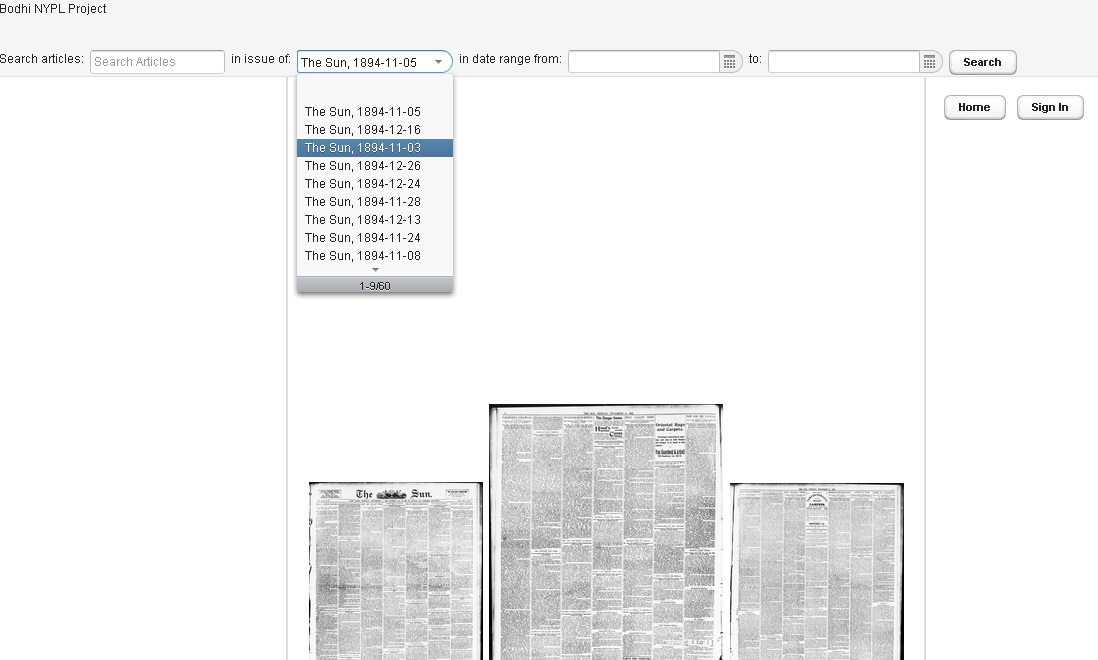
\includegraphics[width=14cm,height=8cm]{C:/Users/Megha/Documents/LEdProjects/ScholarlyMT11024/dropdown.jpg}
\caption{List of issues}
\label{fig:Phase 1}
\end{figure}

\begin{figure}[H]
\centering
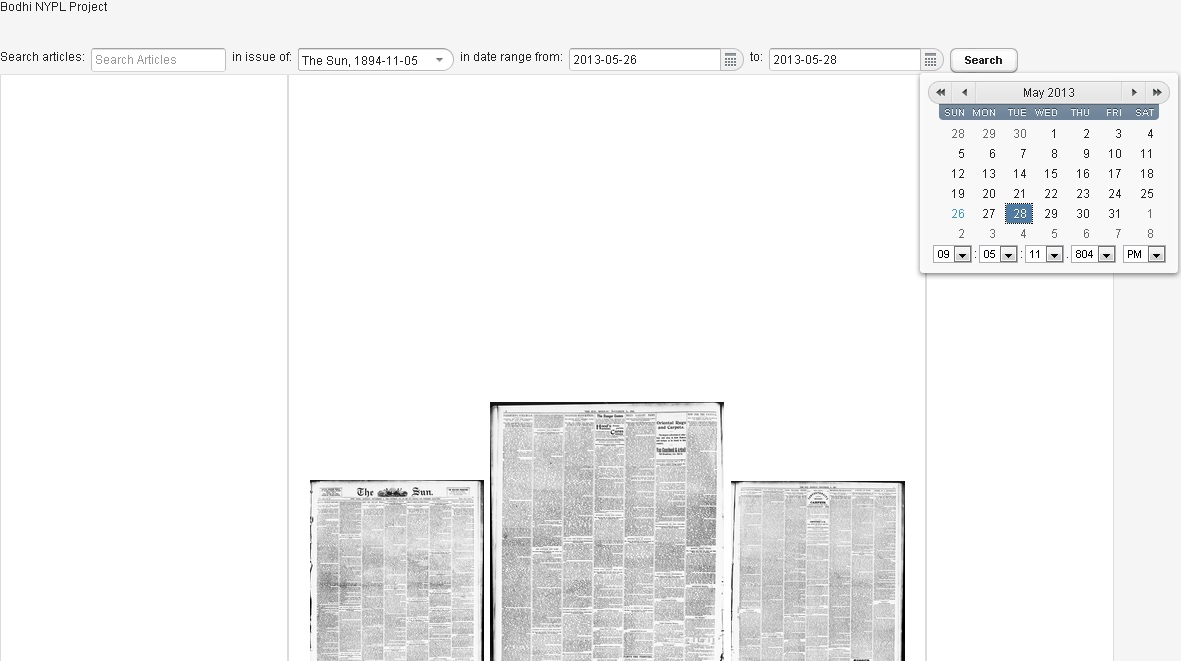
\includegraphics[width=14cm,height=8cm]{C:/Users/Megha/Documents/LEdProjects/ScholarlyMT11024/datepicker.jpg}
\caption{Datepicker}
\label{fig:Phase 1}
\end{figure}

\begin{figure}[H]
\centering
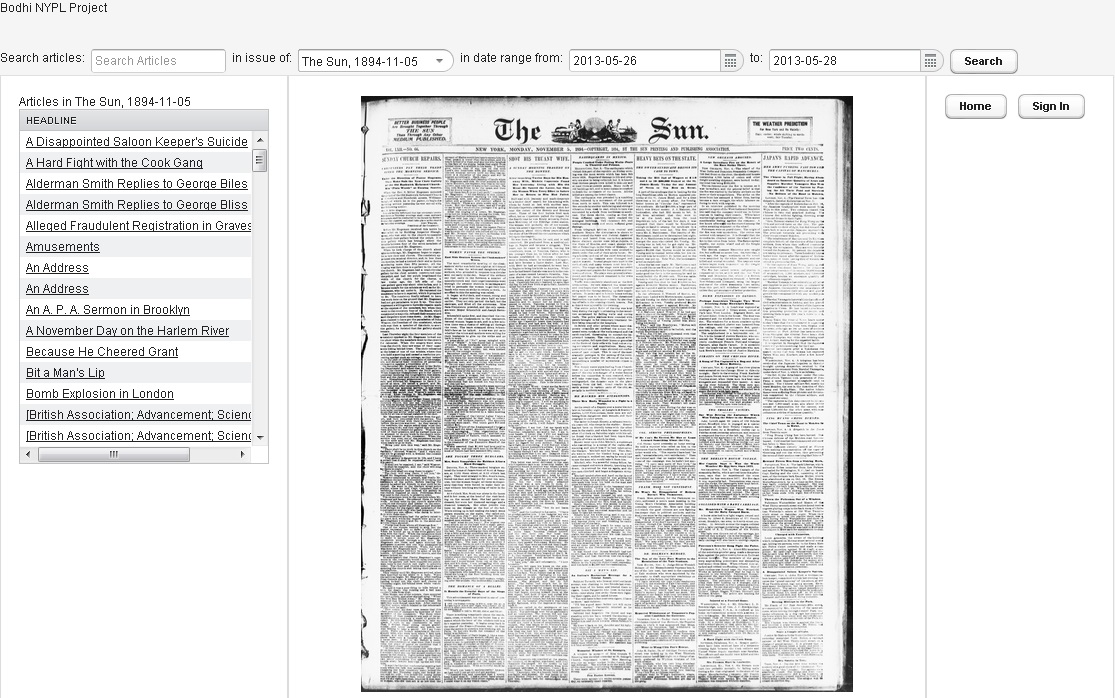
\includegraphics[width=14cm,height=8cm]{C:/Users/Megha/Documents/LEdProjects/ScholarlyMT11024/results.jpg}
\caption{List of headlines in a issue}
\label{fig:Phase 2}
\end{figure}

\begin{figure}[H]
\centering
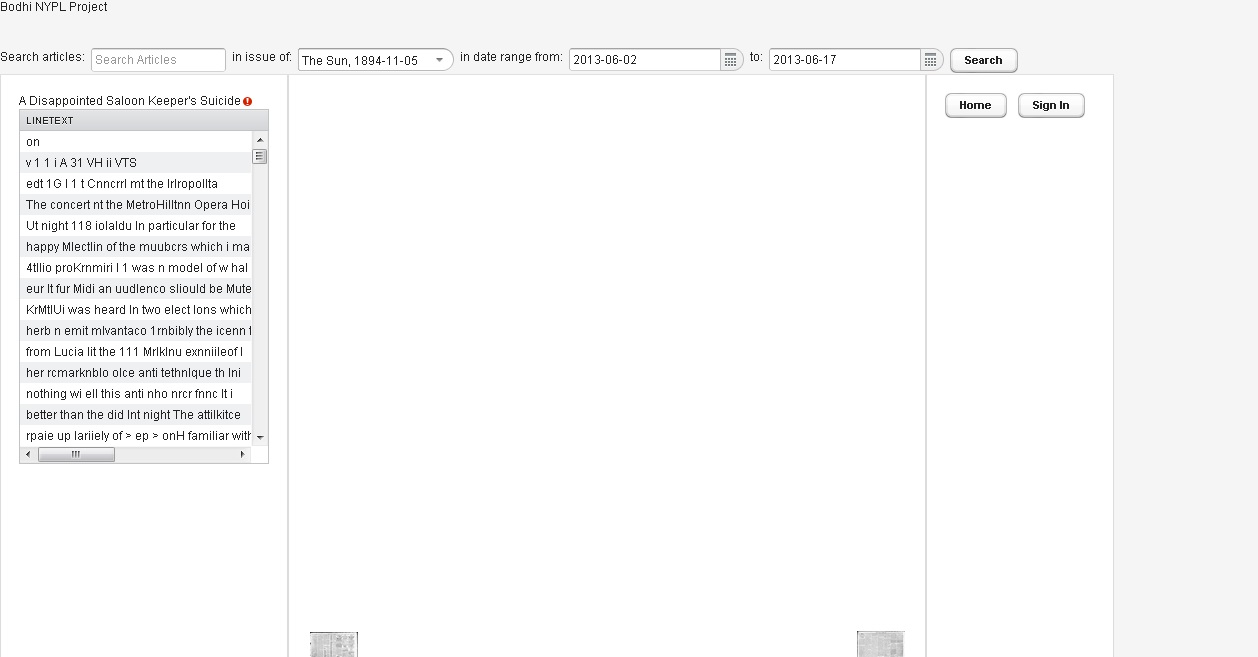
\includegraphics[width=14cm,height=8cm]{C:/Users/Megha/Documents/LEdProjects/ScholarlyMT11024/ocr_text.jpeg}
\caption{OCR text of a particular headline}
\label{fig:Phase 2}
\end{figure}

\begin{figure}[H]
\centering
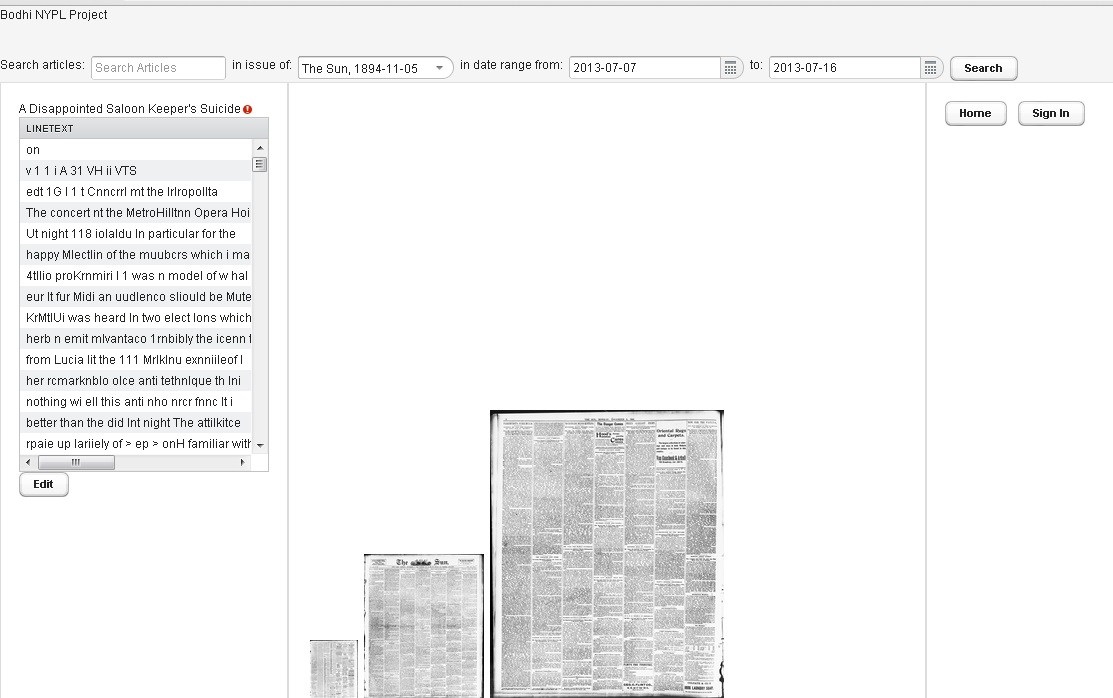
\includegraphics[width=14cm,height=8cm]{C:/Users/Megha/Documents/LEdProjects/ScholarlyMT11024/editscreen.jpg}
\caption{Edit button to edit OCR Text}
\label{fig:Phase 2}
\end{figure}

\subsection{Challenges}
There were several challenges faced during the project, few of them are listed below.
\begin{enumerate}
\item Firewall at server end: Since the database server was at an external location secured with firewall, there were problems in accessing the server at first.
\item Firewall at client end: After the access was granted the problem arose at my end due to Cyberoam layer. I could access the server from outside but not institution due to restricted remote access in the presence of firewall. Finally I was allotted a port using which I could successfully create a secure tunnel.
\item Inaccessible Images: Images that were to be displayed in the web page were not available publicly as they were present only on the server. So hundreds of images of size 3.5GB were first securely copied (PSCP) to the client and then they were pushed to the cloud.
\item Incompatible Images: All the images that were available were of the format .jp2 which is JPEG 2000. It uses a wavelet compression algorithm instead of the common DCT compression method that is used with standard JPEG images.\\
This format can be used to store either lossy or lossless compressed JPEG images and provides the user with a better quality and smaller file size than the traditional JPG image files.\\
But these images are not supported by the browser, hence they can not be opened in the browser.
\item Long delays : When instead of using JPEG 2000 which does not open in any browser, we use JPEG images with each image size of around 5-6 MB, the server tends to hang due to large size of the image. Longer delays are experienced to retrieve Raw OCR Text.
\end{enumerate}

\section{Conclusion}
The OCR \cite{OCR} Text Correction System has not been fully implemented yet. There are several challenges as described above that require attention before proceeding further in terms of implementation. This system when functional will contain a repository of articles which would be clean and usable by many. The process of editing text will also help in building and growing of a community.\\
Once the system would be functional, it will certainly act as a rich source of information for historians, researchers, scholars and users in general.\\

\section{Acknowledgement}
This implementation project was a part of my MTech Scholarly work. I would like to express my gratitude to both my Advisors Dr. Haimonti Dutta and Manoj Pooleery for their constant support and guidance without which I would have never been able to complete it.

\nocite{cdnc,digital,eval,noisy}

\section{Bibiliography}
\bibliography{Scholarly_report}
\bibliographystyle{plain}


\end{document}
